\section{Library Learning over Terms}\label{sec:au}

In this section
  we formalize the problem of
  library learning over a corpus of terms and
  motivate our first core contribution:
  generating candidate abstractions via anti-unification.
%
\autoref{sec:egraphs} generalizes this formalism to library learning over an e-graph.
%
For simplicity of exposition,
our formalization of library learning is \emph{first order},
that is, the initial corpus does not itself contain any $\lambda$-abstractions,
and all the learned abstractions are first-order functions
(the \tool implementation does not have this limitation).

% The goal of this section is to formalize the core algorithm of LLMT---%
% e-graph anti-unification---%
% and to show that this algorithm is complete as a candidate generator for library learning:
% that is, it does not discard optimal candidate abstractions.
% %
% We first consider library learning over a term
% and then generalize to an e-graph.
% We build up to the full algorithm in steps:
% starting with abstracting two terms at the top level,
% and then generalizing to all subterms in a program,
% and finally to all e-classes in an e-graph.

\subsection{Preliminaries}

\mypara{Terms}
%
A \emph{signature} $\Sigma$ is a set of constructors,
each associated with an arity.
%
$\termsof{\Sigma}$ denotes the set of \emph{terms} over $\Sigma$,
defined as the smallest set containing all $s(t_1,\dots,t_k)$
where $s \in \Sigma$, $k = \arity(s)$, and $t_1,\dots,t_k\in\termsof{\Sigma}$.
%
We abbreviate nullary terms of the form $s()$ as $s$.
%
The \emph{size} of a term $\sz(t)$ is defined in the usual way
(as the number of constructors in the term).
%
We use $\subterms(t)$ to denote the set of all subterms of $t$ (including $t$ itself).
%
We assume that $\Sigma$ contains a dedicated \emph{variadic} tuple constructor,
written $\langle t_1, \ldots, t_n \rangle$,
which we use to represent a corpus of programs as a single term
($\langle \rangle$ does not contribute to the size of a term).

\mypara{Patterns}
%
If $\mathcal{X}$ is a denumerable set of variables,
$\patsof{\Sigma}{\mathcal{X}}$ is a set of \emph{patterns},
\ie terms that can contain variables from $\mathcal{X}$.
%
A pattern is \emph{linear} if each of its variables occurs only once:
$\forall X \in \fv(p) . \occ(X, p) = 1$.
%
A \emph{substitution} $\sigma = [\subst{X_1}{p_1}, \ldots, \subst{X_n}{p_n}]$
is a mapping from variables to patterns.
%
% We are often interested in \emph{grounding substitutions},
% where all right-hand sides are terms.
% that maps each $X_i$ to $p_i$ and is identity elsewhere.
%
We write $\sapp{\sigma}{p}$ to denote the application of $\sigma$ to pattern $p$,
which is defined in the standard way.
%
We define the size of a substitution $\sz(\sigma)$ as the total size of its right-hand sides.

A pattern $p$ is more general than (or \emph{matches}) $p'$,
written $p' \sub p$,
if there exists $\sigma$ such that $p' = \sapp{\sigma}{p}$;
we will denote such a $\sigma$ by $\match{p'}{p}$.
%
For example $X + 1 \sub X + Y$ with $\match{X + 1}{X + Y} = [\subst{Y}{1}]$.
%
The relation $\sub$ is a partial order on patterns,
and induces an equivalence relation $p_1 \sim p_2 \triangleq p_1 \sub p_2 \wedge p_2 \sub p_1$
(equivalence up to variable renaming).
%
In the following, we always distinguish patterns only up to this equivalence relation. 

The \emph{join} of two patterns $p_1 \join p_2$---also called their \emph{anti-unifier}---%
is the least general pattern that matches both $p_1$ and $p_2$;
the join is unique up to $\sim$.
%
Note that $\langle \patsof{\Sigma}{\mathcal{X}}, \sub, \join, \top = X \rangle$ is a join semi-lattice
(part of Plotkin's \emph{subsumption lattice}~\cite{plotkin1970lattice}).
%
Consequently, the join can be generalized to an arbitrary set of patterns.

A \emph{context} $\ctx$ is a pattern with a single occurrence of a distinguished variable $\circ$.
%
We write $\ctx[p]$---$p$ in context $\ctx$---as a syntactic sugar for $\sapp{[\subst{\circ}{p}]}{\ctx}$.
%
A \emph{rewrite rule} $R$ is a pair of patterns, written $p_1 \Rightarrow p_2$.
%
Applying a rewrite rule $R$ to a term or pattern $p$, written $\sapp{R}{p}$ is defined in the standard way:
$\sapp{R}{p} = \sapp{(\match{p}{p_1})}{p_2}$ if $p \sub p_1$ and undefined otherwise.
%
A pattern $p$ can be \emph{re-written in one step} into $q$ using a rule $R$,
written $p \rwsteps{R} q$, 
if there exists a context $\ctx$ such that $p = \ctx[p']$ and $q = \ctx[\sapp{R}{p'}]$.
%
The reflexive-transitive closure of this relation is the \emph{rewrite relation} $\rewrites{\ruleset}$,
where $\ruleset$ is a set of rewrite rules.

\mypara{Compressed Terms}
%
Compressed terms $\absof{\Sigma}{\mathcal{X}}$ are of the form:
$$
\hat{t} ::= X   \mid   s(\hat{t}_1,\ldots,\hat{t}_k)     \mid (\lambda X_1 \ldots X_n \bnd \hat{t})\ \hat{t}_1\ \ldots\ \hat{t}_n  
$$
In other words,
compressed terms may contain applications of a $\lambda$-abstraction with zero or more binders
to the same number of arguments.
%
Note that this is a first-order language in the sense that all abstractions are fully applied.
%
  % \footnote{Hereafter, $\many{a}$ stands for a sequence of elements of syntactic class $a$ and $\emptyseq$ denotes the empty sequence.}  
%  compressed terms may have lambdas,
%  which \emph{may} reduce the overall size of the term
%  if the same function is used in multiple locations. 
%
Importantly, we define $\sz(\hat{t})$ in such a way 
that multiple occurrences of a $\lambda$-abstraction are \emph{only counted once}.
% as a result, introducing abstractions may reduce the overall size of the term
% if the same function is used in multiple locations. 
%
For simplicity of accounting, the size of an application $(\lambda \many{X} \bnd \hat{t}_1)\ \many{\hat{t}_2}$
is defined as $\sz(\hat{t}_1) + \sum{\many{\sz(\hat{t}_2)}}$,
that is, abstraction nodes themselves do not add to the size.%
\footnote{Hereafter, $\many{a}$ stands for a sequence of elements of syntactic class $a$ and $\emptyseq$ denotes the empty sequence.}  

% (but this does not make any qualitative difference).
%
% We introduce the standard syntactic sugar $\lambda \many{X} \bnd \hat{t}$%
% for nested abstractions,
% $\hat{t}\ \many{\hat{t}}$ for nested applications,
% and $\T{let}\ X = \hat{t}_1\ \T{in}\ \hat{t}_2$
% for $(\lambda X \bnd \hat{t}_2)\ \hat{t}_1$.

\emph{Beta-reduction} on compressed terms, denoted $\hat{t}_1 \betared \hat{t}_2$, is defined in the usual way:
\[
  (\lambda \many{X} \bnd \hat{t}_1)\ \many{\hat{t}_2}  \betared \sapp{[\many{X \mapsto \hat{t}_2}]}{\hat{t}_1} 
\]
%
where substitution on compressed terms is the standard capture-avoiding substitution for $\lambda$-calculus.
%
Note that because our language is first-order and has no built-in recursion,
it is strongly normalizing
(the proof of this statement, as well as other proofs omitted from this section, can be found in the supplementary material).
%
Hence, the order of $\beta$-reductions is irrelevant,
and without loss of generality we can define \emph{evaluation} on compressed terms, $\hat{t}_1 \evals \hat{t}_2$,
to follow applicative order, \ie innermost $\beta$-redexes are reduced first.
%
As a result, any application reduced during evaluation
has the form $(\lambda \many{X} \bnd p_1)\ \many{p_2}$,
that is, neither the body $p_1$ nor the actual arguments $\many{p_2}$ contain any redexes
(and hence any $\lambda$-abstractions).
%
This simplifies several aspects of our formalization;
for example, there is no need for $\alpha$-renaming, 
since with no binders in $p_1$, no variable capture can occur.


\mypara{Problem Statement}
%
% We will say that $\hat{t} \in \absof{\Sigma}{\mathcal{X}}$ 
% is a \emph{compression of} the term $t \in \termsof{\Sigma}$ 
% if $\hat{t} \evals t$ 
% ($\hat{t}$ evaluates to $t$).
%
We can now formalize
  the \emph{library learning problem} as follows:
  given a term $t \in \termsof{\Sigma}$,
  the goal is to find the smallest compressed term $\hat{t} \in \absof{\Sigma}{\mathcal{X}}$
  that evaluates to $t$ (\ie $\hat{t} \evals t$).
%  
The reason such $\hat{t}$ may be smaller than $t$,
  is that it may contain multiple occurrences of the same $\lambda$-abstraction
  (applied to different arguments),
  whose size is only counted once.
%
An example is shown
  in \autoref{fig:lib-learning-example}.

Although in full generality the solution might include nested lambdas with free variables
(defined in the outer lambdas),
in the rest of the paper we restrict our attention to \emph{global library learning},
where all lambdas are closed terms.
%
This is motivated by the purpose of library learning
to discover reusable abstraction for a given problem domain.
%
The solution in \autoref{fig:lib-learning-example} already has this form.

\begin{figure}
  \begin{minipage}{.5\textwidth}
    \begin{align*}
      \langle &f(g(a) + g(a)) + (g(1) + h(2))\\
      ,\ &f(g(b) + g(b)) + (g(3) + h(4))\\
      ,\ &g(5) + h(6) \rangle
    \end{align*}
  \end{minipage}%
  \begin{minipage}{.5\textwidth}
    \begin{align*}
      &\langle \hat{f}_2\ g(a)\ 1\ 2, \hat{f}_2\ g(b)\ 2\ 3, \hat{f}_1\ 5\ 6\rangle\quad \text{where}\\
      &\hat{f}_1 = \lambda Y\ Z \bnd g(Y) + h(Z)\\
      &\hat{f}_2 = \lambda X\ Y\ Z \bnd f(X + X) + \hat{f}_1\ Y\ Z
    \end{align*}
  \end{minipage}
  \caption{Library learning.
           Left: initial term (size 29).
           Right: an optimal solution with two abstractions, one of which uses the other (size 26).
           A solution with $\hat{f}_2 = \lambda X\ Y\ Z \bnd f(g(X) + g(X)) + \hat{f}_1\ Y\ Z$ also has size 26.}\label{fig:lib-learning-example}
\end{figure}


\subsection{Pattern-Based Library Learning}

At a high-level, our approach to library learning
is to use \emph{patterns} that occur in the original corpus
as candidate bodies for $\lambda$-abstractions in the compressed corpus.
%
Looking at the example in \autoref{fig:lib-learning-example},
it is not immediately obvious that using just the patterns from the original corpus is sufficient,
since the body of $f_2$ contains an application of $f_1$.
%
Perhaps surprisingly, this is not an issue:
the key idea is that we can compress $t$ into $\hat{t}$ by inverting the evaluation $\hat{t} \evals t$,
and because the evaluation order is applicative,
the rewritten sub-term at every step will not contain any $\beta$-redexes.

\mypara{Compression}
%
More formally, given a pattern $p$,
let us define its \emph{compression rule} (or $\kappa$-rule for short)
as the rewrite rule
\[
  \kappa(p) \; \triangleq \; p \Rightarrow (\lambda \many{X} \bnd p)\ \many{X} \quad \text{where}\quad \many{X} = \fv(p)
\]
%
In other words, $\kappa(p)$ will replace any term 
matching $p$ with an application of a function whose body is \emph{exactly} $p$.
%
For example, if $p = g(Y) + h(Z)$,
its $\kappa$-rule is $g(Y) + h(Z) \Rightarrow (\lambda Y\ Z \bnd g(Y) + h(Z))\ Y\ Z$.
%
Note that on the right-hand side of this rule 
only the \emph{free} occurrences of $Y$ and $Z$ will be substituted during rewriting;
the bound $Y$ and $Z$ will be left unchanged, following the usual semantics of substitution for $\lambda$-calculus.
%
For example, this rule can rewrite the third term in \autoref{fig:lib-learning-example} (left) as follows:
\[
  g(5) + h(6) \;\rwsteps{\kappa(g(Y) + h(Z))}\; (\lambda Y\ Z \bnd g(Y) + h(Z))\ 5\ 6
\]
%
% We will refer to a rewrite step such as the one above as a $\kappa$-step.
%
A sequence of $\kappa$-rewrites $t \rwsteps{\kappa(p_1)} \dots \rwsteps{\kappa(p_n)} \hat{t}$,
where all $p_i \in \patset$, 
is called a \emph{compression} of $t$ into $\hat{t}$ using patterns $\patset$
and written $t \rewrites{\kappa(\patset)} \hat{t}$.
%
We can now show that the library learning problem is equivalent to finding the smallest compression of $t$
using only patterns that occur in $t$.

\begin{theorem}[Soundness and Completeness of Pattern-Based Library Learning]
  For any term $t \in \termsof{\Sigma}$ and compressed term $\hat{t} \in \absof{\Sigma}{\mathcal{X}}$:
  \begin{description}[font=\itshape]
    \item[(Soundness)] If $t$ compresses into $\hat{t}$, then $\hat{t}$ evaluates to $t$: $\forall \patset . t \rewrites{\kappa(\patset)} \hat{t} \Longrightarrow \hat{t} \evals t$.
    \item[(Completeness)] If $\hat{t}$ is a solution to the (global) library learning problem, 
    then $t$ compresses into $\hat{t}$ using only patterns that have a match in $t$:
    $\hat{t} \in \argmin_{\hat{t}' \evals t} \sz(\hat{t}') \Longrightarrow t \rewrites{\kappa(\patset)} \hat{t}$, 
    where $\patset = \{p \in \patsof{\Sigma}{\mathcal{X}} \mid t' \in \subterms(t) , t' \sub p\}$.
  \end{description}
\label{thm:pat-lib-learning}
\end{theorem} 
%
The proof can be found in the supplementary material. % \autoref{app:proofs}.

\mypara{Example}
%
Consider once again the library learning problem in \autoref{fig:lib-learning-example}.
%
Here the set of patterns used to compress the original corpus into the solution on the right is:
\[
  p_1 = g(Y) + h(Z)\quad\quad\quad
  p_2 = f(X + X) + g(Y) + h(Z)
\]
%
Rewriting the first term of the corpus proceeds in two steps (the redexes of $\kappa$-steps are highlighted):
\begin{multline*}
  \textcolor{darkblue}{f(g(a) + g(a)) + (g(1) + h(2))}    \;\rwsteps{\kappa(p_2)}\\     
  (\lambda X\ Y\ Z \bnd f(X + X) + \textcolor{darkblue}{g(Y) + h(Z)})\ g(a)\ g(a)\ (g(1) + h(2))\;\rwsteps{\kappa(p_1)}\\ 
  (\lambda X\ Y\ Z\ \bnd f(X + X) + (\lambda Y\ Z \bnd g(Y) + h(Z))\ Y\ Z)\ g(a)\ g(a)\ (g(1) + h(2))
\end{multline*}
%
In other words, we first rewrite the entire term using $p_2$,
and then rewrite inside the body of the introduced abstraction using $p_1$
(note that this order of compression is the inverse of the applicative evaluation order).
%
The second term of the corpus compresses analogously;
the third term compresses in a single step using $p_1$.
%
Although this is not obvious from the rewrite sequence above,
the resulting compressed corpus is indeed smaller than the original
thanks to sharing of both $\lambda$-abstractions,
as illustrated on the right of \autoref{fig:lib-learning-example}.

\mypara{Library Learning as Term Rewriting}
%
Theorem~\ref{thm:pat-lib-learning} reduces library learning to a \emph{term rewriting} problem.
%
Namely, given a term $t$ and a finite set of rewrite rules $\ruleset = \{\kappa(p) \mid  t' \in \subterms(t) , t' \sub p\}$,
% that consists of $\kappa$-rules for all patterns that have a match in $t$,
our goal is to find a minimal-size term $\hat{t}$ such that $t \rewrites{\ruleset} \hat{t}$,
which is a standard formulation in term rewriting.
%
Unfortunately, this particular problem is notoriously difficult because
(a) the rule set $\ruleset$ is very large for any non-trivial term $t$, and
(b) our $\sz$ function is non-local (it takes sharing into account)
%
In the rest of this section we discuss how we can prune the rule set $\ruleset$ 
to reduce it to a tractable size.
%
\autoref{sec:beam} discusses how we tackle the remaining term rewriting problem
using the \emph{equality saturation} technique~\cite{tate2009equality,willsey2021egg}.


\subsection{Pruning Candidate Patterns}
\label{sec:pruning}

In this section, we discuss which patterns can be discarded from consideration
when constructing the set of $\kappa$-rules $\ruleset$ for the term rewriting problem.

% In this section, 
%  we consider candidate generation
%  starting from the naive but complete
%  approach of generating the infinite set of all patterns $\patsof{\Sigma}{\mathcal{X}}$.
% We show that
%  several classes of patterns are provably suboptimal,
%  eventually reducing the set of viable candidates to a 
%  finite set of patterns that can be enumerated efficiently.

\mypara{Cost of a Pattern}
%
Consider a compression $t \rewrites{\kappa(\patset)} \hat{t}$
where each pattern $p \in \patset$ is used some number $n$ times, 
with substitutions $\sigma^p_1, \ldots, \sigma^p_n$.
%
We can break down the total amount of compression into contributions of individual patterns:
\[
  \sz(\hat{t}) - \sz(t) = \sum_{p \in \patset} \mathsf{cost}(p, \{\sigma^p_1, \dots \sigma^p_n\})
\]
%
The cost of a pattern $p$, in turn, consists of three components.
%
The cost of \emph{introducing} the abstraction is the size of its body, \ie $\sz(p)$.
%
The cost of using an abstraction---%
$\textsf{use}(p, \sigma)$ \eqref{eq:use}---%
 includes the application itself and the size of the arguments.
The cost saved by using an abstraction---%
$\textsf{save}(p, \sigma)$ \eqref{eq:save}---%
 is just the cost of the term matched by $p$
 (\ie the redex of the corresponding $\kappa$-step).
%  rewritten in terms of the size of $p$ itself 
%  and the size of subterms in the substitution.
%
\begin{align}
  % \intro(p) &= \sz(p) \label{eq:intro}\\
  \textsf{use}(p, \sigma) &= 1 + \sum_{X \in \fv(p)} \sz(\sigma(X)) \label{eq:use} \\
  \textsf{save}(p, \sigma) &= \sz(\sapp{\sigma}{p}) = 
  \sz(p) + \sum_{X \in \fv(p)} \occ(X, p) \cdot (\sz(\sigma(X)) - 1)\label{eq:save}
\end{align}
%
The total cost of $p$ is 
 the cost of introducing the abstraction paid a single time,
 plus the cost of each use, minus what you save for each application:
\begin{equation}
  \textsf{cost}(p, \{\sigma_1,\ldots,\sigma_n\}) 
  = \intro(p) + \sum_{\sigma_i} (\textsf{use}(p, \sigma_i) - \textsf{save}(p, \sigma_i))
\end{equation}
%
When $p$ is linear (all $\occ(X, p) = 1$), 
 the cost depends only on $n$ but not on the substitutions $\sigma_i$:
\begin{align}
  \textsf{cost}(p, \{\sigma_1,\ldots,\sigma_n\}) 
  &= \intro(p) + \sum_{\sigma_i} \left(
    1 - \sz(p) + |\fv(p)|
  \right) \\
  &= \intro(p) + n \cdot \left(
    1 - \sz(p) + |\fv(p)|
  \right)
\end{align}
%
We can show that a pattern $p$ with a \emph{non-negative} cost can be safely discarded,
that is: there exists another compression using only $\patset \setminus \{p\}$,
whose result is at least as small.
% A pattern is only worth including into the compression if its \textsf{cost} is negative.

\mypara{Trivial Patterns}
%
Based on this analysis, any linear pattern $p$
 with $\sk(p) \leq 1$ can be discarded,
 where $\sk(p) = \sz(p) - |\fv(p)|$ is the size of $p$'s ``skeleton'', \ie it's body without the variables.
%
Intuitively, the skeleton of $p$ is simply too small to pay for introducing an application.
%
In this case, $\mathsf{cost}(p,\_) > 0$ \emph{independently} of how many times it is used.
%
We refer to such patterns as \emph{trivial}.
%
Examples of trivial patterns are $X$ and $X + Y$.


% \mypara{Patterns with No Matches}
% %
% Like in prior work~\cite{dreamcoder},
% we can trivially discard patterns that do not match any subterm of $t$
% (where $n=0$ above).
% %
% In this case we only pay for adding a definition,
% but never get to gain from applying it,
% so such a pattern clearly cannot be part of an optimal solution.

\mypara{Patterns with a Single Match}
%
We can show that patterns with only a single match in the corpus can also be discarded.
%
If $p$ has a single match in $t$,
then it can appear \emph{at most once} in any compression of $t$.
%
If $p$ is linear, $\mathsf{cost}(p, \_) = 1 + |\fv(p)|$,
which is always positive, so $p$ can be discarded.
%
But what about non-linear patterns, where even a single $\kappa$-step can decrease size thanks to variable reuse?
%
It turns out that any non-linear pattern with a single match
can always be replaced by a nullary pattern (with no variables) that is more optimal.

Without loss of generality, assume that $p$ has a single variable $X$ that occurs $m > 1$ times,
and let its sole $\kappa$-step be $\sapp{\sigma}{p} \rwsteps{\kappa(p)}  (\lambda X \bnd p)\  \sapp{\sigma}{X}$.
%
The size of the right-hand side is $\sz(p) + 1 + \sz(\sapp{\sigma}{X})$,
or, rewritten in terms of $p$'s skeleton: $1 + (\sk(p) + m) + \sz(\sapp{\sigma}{X})$.
%
Instead, we can rewrite the same redex $\sapp{\sigma}{p} \rewrites{\{R\}} p'$
using $m$ applications of the rule $R \;\triangleq\; \sapp{\sigma}{X} \Rightarrow (\lambda \epsilon \bnd \sapp{\sigma}{X})\ \epsilon$.
%
This is a $\kappa$-rule for a \emph{nullary} pattern $\sapp{\sigma}{X}$ with no variables
(hence the corresponding $\lambda$-abstraction has zero binders).
%
The size of $p'$ obtained in this way is $\sz(\sapp{\sigma}{X}) + m + \sk(p)$
(where the former is the size of the shared $\lambda$-abstraction, $m$ is the number of applications, 
and $\sk(p)$ is the size of the term around the applications).
%
As you can see, this term is one smaller than the one we get by applying $p$.
%
Intuitively, this result says that instead of using a non-linear pattern that occurs only once,
it is better to perform common sub-expression elimination.

% \mypara{Minimal Generalization}
% %
% Consider two patterns $p$ and $p'$ with the same matches in the corpus,
% such that $p$ is more general than $p'$.
% %
% It might seem in this case that $p$ can be pruned
% (because $p'$ factors out more of the common structure of the matched terms),
% but this is not always the case.
% %
% Consider the following corpus:
% \begin{equation}
%   \langle t_1, t_2\rangle \quad\text{where}\ t_i = f(g(h(t'_i))) + f(g(h(t'_i))) + f(g(h(t'_i)))
%   \label{eq:cex}
% \end{equation}
% and $t'_1$ and $t'_2$ are some terms of size 5, with different root constructors;
% this corpus has size $26*2 = 52$.
% %
% Consider the following two patterns:
% \[
%   p = X + X + X
%   \quad\quad\quad 
%   p' = f(g(h(X))) + f(g(h(X))) + f(g(h(X))) 
% \]
% Both of them have exactly two matches in the corpus and $p \sub p'$;
% yet compressing the corpus using $p$ has size 23 and compressing it using $p'$ has size 26:
% \begin{align*}
% \T{let}\ P =& X + X + X\ \T{in}\ \langle P\ (f(g(h(t'_1)))), P\ (f(g(h(t'_2)))) \rangle  \\  
% \T{let}\ P =& f(g(h(X))) + f(g(h(X))) + f(g(h(X)))\ \T{in}\ \langle P\ t'_1, P\ t'_2 \rangle
% \end{align*}
% %
% The issue is that although the applications of $p'$ are smaller, 
% the pattern itself is much larger.

% This example, however, gives us a clue for when a more general pattern \emph{can} be pruned.
% %
% We say that $p$ is a \emph{minimal generalization} of $p'$
% if $p$ abstracts over a sub-pattern of $p'$, 
% and all occurrences of that sub-pattern are abstracted into the same variable.
% %
% For example, both patterns $X + X + Y$ and $f(g(h(X))) + X + X$ are \emph{not} minimal generalization of $p'$
% and they are both clearly suboptimal compared to a minimal generalization $p$:
% they are no smaller than $p$, and their applications need at least the same set of actual arguments.

% There is one special case, however, where we can discard the more general pattern:
% where the substitution $\match{p'}{p}$ simply renames variables;
% for example, although the pattern $X + X + X$ is useful in the example above,
% the more general pattern $X + X + Y$ is definitely not useful.
% %
% This is because in this case $\sz(p) = \sz(p')$,
% but every application of $p$ must have a superset of the actual arguments.
% %
% In other words, for a more general pattern $p$ to be useful,
% it must abstract over some \emph{non-trivial subterm} of $p'$,
% not just a single variable.

% \begin{figure}
%   $$
%   \begin{array}{rl}
%     \gau(s(t_1,\ldots,t_k), s(t'_1,\ldots,t'_k)) &= \textcolor{darkblue}{\{X_{s(\ldots),s(\ldots)}\} \cup} \{s(p_1,\ldots,p_k) \mid p_i \in \gau(t_i,t'_i)\}\\
%     \gau(s_1(\ldots),s_2(\ldots)) &= \{X_{s_1(\ldots),s_2(\ldots)}\} \quad\text{if}\ s_1 \neq s_2
%     \end{array}
%   $$
% \caption{Generalizing anti-unification of two terms.}\label{fig:gau}
% \end{figure}

% \subsection{Generalizing Anti-Unification}

\mypara{Parameterization Lattice}
%
Eliminating from consideration all patterns with fewer than two matches in the corpus
suggests an algorithm for generating a complete set $\patset$ of candidate patterns:
  (1) start from the set $\plau{t} = \{t_1 \join t_2 \mid t_i \in \subterms(t)\}$
      of all pairwise joins of subterms of the input program,
  (2) explore all elements of the subsumption semi-lattice above those patterns,
      by gradually replacing sub-patterns with variables,
      until we hit trivial patterns at the top of the lattice.
%
We will refer to this semi-lattice above $\plau{t}$ as the \emph{parametrization lattice} of $t$, 
denoted $\pl{t}$.
%
A fragment of $\pl{t}$ for $t = \langle f(a+b), f(a+c), f(b+c)\rangle$ is shown in \autoref{fig:lattice} (left).


% The lattice $\pl{t}$ gives us an algorithmic way of exploring the space of viable patterns:
% (1) start by computing $\plau{t}$ by anti-unifying all pairs of subterms of $t$, then
% (2) traverse the lattice upwards by gradually replacing sub-patterns with variables,
% until we hit trivial patterns at the top of the lattice.

% The discussion above suggests the following definition of the set of candidate patterns $\pl{t}$ for compressing a term $t$:
% $\pl{t}$ must include all pairwise joins of subterms of $t$ and all their minimal generalizations
% (except if any of these patterns is trivial).

% To compute $\pl{t}$, we define \emph{generalizing anti-unification} $\gau(t_1, t_2)$, 
% which takes two terms and computes a set of patterns,
% consisting of their join and all its minimal generalizations.
% %
% This function is formalized in \autoref{fig:gau}.
% %
% The main difference from traditional term anti-unification is highlighted in blue:
% when the root constructor of two terms is the same,
% $\gau$ still includes a a variable (in addition to recursing into subterms);
% this enables $\gau$ to include minimal generalizations of join.
% %
% Note that unlike some traditional presentations of anti-unification,
% we do not keep track of the anti-substitution 
% to avoid abstracting the same pairs of terms into different variables;
% instead we achieve the same effect simply by naming the variables $X_{t_1,t_2}$
% after the pair of terms they abstract.


\begin{figure}
  \begin{minipage}{.5\textwidth}
    \centering
    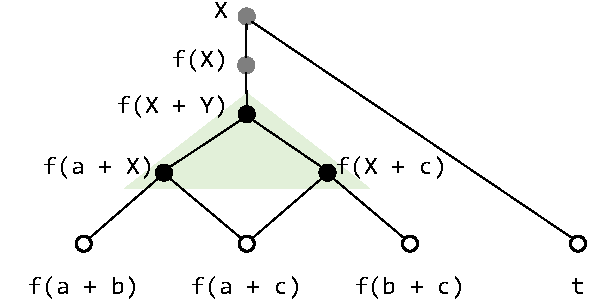
\includegraphics[width=.8\textwidth]{figures/lattice-1.pdf}      
  \end{minipage}%
  \begin{minipage}{.5\textwidth}
    \centering
    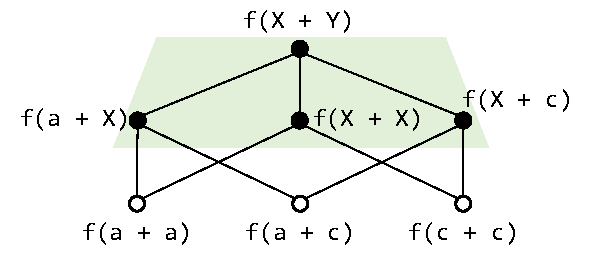
\includegraphics[width=.8\textwidth]{figures/lattice-2.pdf}      
  \end{minipage}
  \caption{Left: fragment of the parametrization lattice for the term $t = \langle f(a+b), f(a+c), f(b+c)\rangle$;
           only filled black circles correspond to candidate patterns:
           hollow circles match fewer than two terms and gray circles are trivial.
           Right: an example where is it insufficient to consider pairwise joins
           to obtain an optimal pattern.}
  \label{fig:lattice}
\end{figure}


% \autoref{fig:lattice} illustrated generalizing anti-unification on two examples.
% %
% The example on the left is a simplified version of \eqref{eq:cex}:
% here we see that $\gau$ includes the optimal pattern $X + X$
% (because $X \in \gau(f(g(t_1)), f(g(t_2)))$).
% %
% The example on the right is a well-known example where the join of three terms is different from all their pairwise joins;
% here we can see that pairwise generalizing anti-unification is still able to recover the three-way join.
% %
% \TODO{Can we say anything why this is generally true?} 


% \mypara{Overly General Linear Patterns}
% %
% For linear patterns, we can in fact show that any pattern that is not a join of some subset of $\subterms(t)$
% can be discarded;
% for example, this applies to patterns $f(X)$ and $X$ in \autoref{fig:lattice} (left).%
% \footenote{In this particular case, both patterns are also trivial, but the same reasoning would apply to non-trivial patterns.}

% Consider two patterns $p, p'$, such that $p' = \join(t_1, \ldots, t_2)$, $p \sub p'$, $p$ is linear,
% but $p$ does not match any other subterms of $t$ ($\forall t'\in \subterms(t) . p \sub t' \Longrightarrow t' \in \{t_1, \ldots, t_2\}$).
% %
% We can show that $p$ can always we replaced with $p'$ during library learning without increasing cost.
% %
% The key observation is that because $p$ does not match any other subterms,
% they both can be applied the same number of times $n \geq 2$.
% %
% The goal is to show that while $p$ can be smaller than $p'$,
% each of its applications does not provide as much savings as the corresponding application of $p'$,
% and since there are at least two applications, they can always make up for the difference in the pattern size.
% %
% \TODO{I managed to prove that the different in size between compressing with $p$ and $p'$ is greater equal than
% $\sz(\sigma) + |\fv(p)| - 2|\fv(p')|$}, where $\sigma = \match{p}{p'}$
% and assuming (without loss of generality) that $\fv(p) \cap \fv(p') = \emptyset$; why is this always non-negative?}

\mypara{Approximation}
%
In practice, computing the set $\plau{t}$ is feasible:
although there are quadratically many pairs of subterms,
most of them do not have a common constructor at the root, and hence their join is trivially $X$.
%
An example is the join of $t$ with any of its subterms in \autoref{fig:lattice} (left).
%
Unfortunately, generalizing the patterns from $\plau{t}$ 
according to the parameterization lattice (\autoref{fig:lattice}) is expensive.
%
For this reason, \tool adopts an approximation
and simply uses $\plau{t}$ as the set of candidates.

This approximation makes our pattern generation theoretically incomplete.
%
Consider a pattern $p \in \pl{t}\setminus \plau{t}$;
%% Nadia: actually, another case if when a more concrete pattern would block a later compression of actual args: is this a real thing?
there are two reasons why we might need $p$ in the optimal compression of $t$:
\begin{enumerate}
  \item there is \emph{no} $p' \in \plau{t}$ with the same set of matches as $p$, or
  \item there is such a $p'$ but it has \emph{few enough matches} 
  that its larger size does not pay off. 
  % despite a lower use cost per match.
\end{enumerate}
%
% Let us consider both options in more detail.

The first kind of incompleteness occurs when $p$ matches a set of subterms $t_1, \ldots, t_n$ ($n > 2$),
whose join is distinct from all their pairwise joins
(otherwise some $t_i \join t_j \in \plau{t}$ would also match all $t_1, \ldots, t_n$).
%
An example is shown in \autoref{fig:lattice} (right),
where the three subterms in question are $f(a+a)$, $f(a+c)$, and $f(c+c)$.
%
In this case, an optimal compression might use the pattern $f(X+Y)$ to rewrite all three subterms,
but our approximation would only include the patterns $f(a+X)$, $f(X+X)$, and $f(X+c)$,
each of which can rewrite only two of the three subterms.

The second kind of incompleteness occurs when there exists $p' \in \plau{t}$
that has the same set of matches as $p$, despite being strictly more specific,
and yet using $p'$ instead of $p$ still doe not pay off.
%
The understand when this happens, consider the difference in costs between $p$ and $p'$, 
assuming that they are both used to rewrite the same $n$ subterms
(\ie their \textsf{save} cost is the same):
\begin{align*}
  \mathsf{cost}(p', \many{\sigma'}) - \mathsf{cost}(p, \many{\sigma}) &= \sz(p') - \sz(p) + \sum_i (\mathsf{use}(p', \sigma'_i) - \mathsf{use}(p, \sigma_i))\\
  &= \sz(p') - \sz(p) + \sum_i (\sz(\sigma'_i) - \sz(\sigma_i))
\end{align*}
%
Because $p'$ is strictly more specific than $p$, we know that $\sz(p') \geq \sz(p)$,
but all its substitutions $\sigma'_i$ must be strictly smaller than $\sigma_i$.
%
Hence, with enough uses, $p'$ is bound to become more compressive than $p$;
when there are just a few uses, however, $p$ can be more optimal.
%
For example, consider the corpus $\langle \ctx[f(1,2,3)],  \ctx[f(4,5,6)]\rangle$,
where $\ctx$ is some sufficiently large context.
%
Here, a more general pattern $p = \ctx[X]$ is more optimal than the more specific $p' = \ctx[f(X,Y,Z)]$,
because $\sz(p') - \sz(p) = 3$, each use of $p'$ is only one node cheaper,
and there are only two uses. 

Despite the lack of theoretical completeness guarantees, 
we argue that restricting candidate patterns to $\plau{t}$ is a reasonable trade-off.
%
Note, that the counter-examples above are quite contrived,
and they no longer apply once the corpus contains sufficiently many and sufficiently diverse instances of a pattern
(for example, adding $f(b,b)$ to the first corpus would make $f(X,Y)$ appear in $\plau{t}$,
and adding just one more occurrence of $p'$ into the second corpus would make it as optimal as $p$).
%
Our empirical evaluation confirms that this approximation works well in practice.

% \subsubsection{Root Abstraction of Two Terms}

% Let us start with the simplest case:
% given two terms $t_1, t_2$,
% we can only abstract at top level,
% that is rewrite into \T{let P = ... in [P[...], P[...]]} or leave as is.
% %
% We claim that the best such $P$ is the anti-unifier of $t_1$ and $t_2$.

% This is not generally true in the presence of \emph{compressive non-linear patterns}.
% %
% Define what it is.
% %
% In this sub-section we exclude such patterns from consideration.
% and in the next section we explain why a compressive linear pattern also cannot be optimal.

% For any given pattern $P$ it either matches none of $t_1, t_2$
% or one of them, or both.
% %
% If it matches none, clearly a waste of space.
% %
% If it matches one, it is also a waste of space because $P$ cannot be non-linear compressive.

% So let's say $P$ matches both terms, and it is optimal,
% but not the AU.
% %
% % This is because the cost of introducing the abstraction is $\sz(P) + \sz(\sigma_1) + \sz(\sigma_2) + 2|\fv(P)| + 1$;
% % $P$ must be an upper bound of $t_1$ and $t_2$.
% %
% We can compute the size difference between rewriting with $P$ and with the AU;
% because non of them are non-linear compressive, the difference is positive.

% \subsubsection{Root Abstraction of $k$ Terms}

% To go from two terms to arbitrary $k$,
% it is clear that we need to partition the terms into clusters that will be abstracted by the same pattern.
% %
% Hence to generate candidates in this case we need to consider AUs of all nontrivial subsets
% (all pairs, all triples, \etc).

% \subsubsection{Abstraction of All Subterms}

% Now we are given a term and we can insert abstractions at any level.
% %
% This amounts to guessing some subsets of sub-terms and then abstracting them at the top-level.
% %
% Hence we can solve this by applying the previous algorithm to all tuples of subterms.
% \TODO{This doesn't seem to properly account for abstractions using other abstractions?}
% %
% In practice this is expensive, and also very rare that the AU of a $k$-tuple of terms
% is not the same as the AU of some pair from that tuple.
% %
% So in practice we restrict to pairs.

% Now let us address why it is okay to not consider compressive non-linear patterns.
% %
% This is because if compression of any subterm requires such pattern,
% it means that this subterms has common sub-expressions of a non-trivial size.
% %
% But in this case, we can first eliminate these common sub-expressions using a free pattern with no variables;
% so we would get the same overall compression but with the non-linear pattern now being non-compressive.

% \TODO{Where do we talk about leaning over terms that already have local bindings?
% This is harder (we need to make sure that patterns don't mention local variables),
% but \tool can do this; although not optimally.}
